\documentclass[10pt]{beamer}

\usepackage[brazilian]{babel}
\usepackage[utf8]{inputenc}
\usepackage{graphicx}
\usepackage{mathtools}
\usepackage{amsthm}
\usepackage{thmtools,thm-restate}
\usepackage{amsfonts}
\usepackage{hyperref}
\usepackage[singlelinecheck=false]{caption}
\usepackage[backend=biber,url=true,doi=true,eprint=false,style=alphabetic]{biblatex}
\usepackage[justification=centering]{caption}
\usepackage{indentfirst}
\usepackage{enumitem}
\usepackage{algorithm}
\usepackage{algpseudocode}
\usepackage{listings}

% Fix beamer and enumitem conflicts.
\setitemize{label=\usebeamerfont*{itemize item}%
  \usebeamercolor[fg]{itemize item}
\usebeamertemplate{itemize item}}

% Remove line breaks.
\setbeamertemplate{bibliography entry title}{}
\setbeamertemplate{bibliography entry location}{}
\setbeamertemplate{bibliography entry note}{}

\uselanguage{Brazilian}
\languagepath{Brazilian}
\usetheme{Berlin}

\addbibresource{references.bib}

\newcommand\nmfootnote[1]{%
  \begingroup
  \renewcommand\thefootnote{}\footnote{#1}%
  \addtocounter{footnote}{-1}%
  \endgroup
}

\makeatletter
\def\subsection{\@startsection{subsection}{3}%
  \z@{.5\linespacing\@plus.7\linespacing}{.1\linespacing}%
  {\normalfont\itshape}}
\makeatother

\DeclareMathOperator*{\argmin}{arg\,min}
\DeclareMathOperator*{\argmax}{arg\,max}

\newcommand\defeq{\mathrel{\overset{\makebox[0pt]{\mbox{\normalfont\tiny\sffamily def}}}{=}}}

\floatname{algorithm}{Algoritmo}
\algrenewcommand\algorithmicrequire{\textbf{Input}}
\algrenewcommand\algorithmicensure{\textbf{Output}}

\captionsetup[table]{labelsep=space}

\theoremstyle{plain}

\newtheorem{proposition}{Proposição}
\newtheorem{exercise}{Exercício}

\newcommand{\set}[1]{\mathbf{#1}}
\newcommand{\pr}{\mathbb{P}}
\renewcommand{\implies}{\Rightarrow}

\newcommand{\bigo}{\mathcal{O}}
\newcommand{\p}{\pause}

\setlength{\parskip}{1em}

\lstset{frameround=fttt,
  language=[5.3]Lua,
  numbers=left,
  breaklines=true,
  keywordstyle=\bfseries,
  basicstyle=\ttfamily,
}

\newcommand\Fontsmall{\fontsize{12}{7.2}\selectfont}

\newcommand{\code}[1]{\lstinline[mathescape=true]{#1}}
\newcommand{\mcode}[1]{\lstinline[mathescape]!#1!}

\title{Estudo sobre Sum-Product Networks e Aprendizagem Profunda}
\author{Renato Lui Geh}
\institute[IME-USP] {%
  Instituto de Matemática e Estatística\\
  Universidade de São Paulo
}
\titlegraphic{\hspace*{7.5cm}~
\includegraphics[scale=0.25]{imgs/logo.png}}

\begin{document}

\frame{\titlepage}

\begin{frame}
  \frametitle{Índice}
  \tableofcontents
\end{frame}

%--------------------------------------------------------------------------------------------------

\section{Motivação}

\begin{frame}
  \frametitle{Outros modelos}
  \begin{itemize}
    \item Redes Bayesianas
    \item Redes de Markov
    \item Máquinas restritas de Boltzmann
  \end{itemize}
  Representam uma distribuição de probabilidade de forma compacta. Mas$\ldots$
  \begin{description}
    \item[Inferência] intratável ou aproximada!
    \item[Aprendizado] difícil!
  \end{description}
\end{frame}

\begin{frame}
  \frametitle{Largura de árvore}
  Largura de árvore grande $\implies$ inferência intratável.
  \begin{figure}[h]
    \centering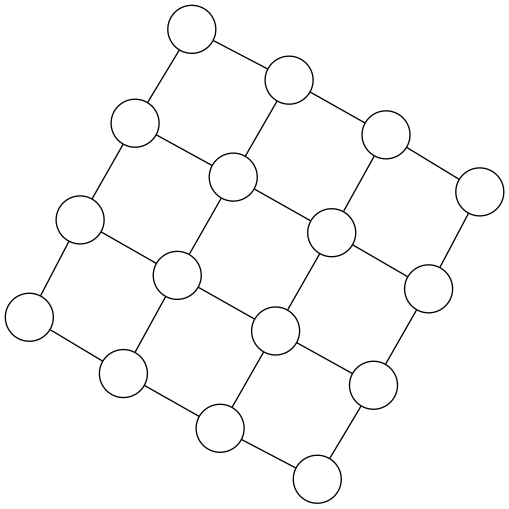
\includegraphics[scale=0.2]{graphs/hightree.png}
    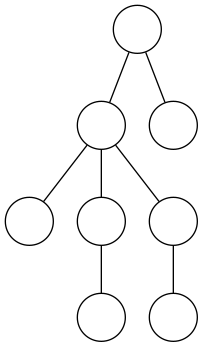
\includegraphics[scale=0.3]{graphs/lowtree.png}
  \end{figure}
  SPNs computam inferência exata e tratável mesmo quando a largura de árvore é grande.
\end{frame}

\begin{frame}
  \frametitle{Arquiteturas profundas}
  \begin{description}
    \item[DBNs:] Deep Belief Networks~\cite{dbns}
    \item[CDBNs:] Convolutional Deep Belief Networks~\cite{cdbns}
    \item[DBMs:] Deep Boltzmann Machines~\cite{dbms}
  \end{description}
  Arquiteturas profundas são mais interessantes~\cite{deep-archs-ai}. Mas$\ldots$
  \begin{description}
    \item[Inferência] mais difícil ainda!
    \item[Aprendizado] mais difícil também!
  \end{description}
\end{frame}

\begin{frame}
  \frametitle{Representatividade}
  \center{%
    1. Modelos tratáveis existentes\\
    vs\\
    2. Modelos baseados em grafos clássicos\\
    vs\\
    3. Redes Soma-Produto (Sum-Product Networks)
  }\\~\\

  1 e 3 ambos tem inferência e aprendizado tratáveis.
  \begin{equation*}
    3 >_g 1
  \end{equation*}
\end{frame}

%--------------------------------------------------------------------------------------------------

\section[SPNs]{Sum-Product Networks}

\begin{frame}
  \frametitle{Definição}
  \begin{definition}\label{gd-def}
    Uma SPN tem uma definição recursiva. Definimos que uma SPN $S_i$ pode ser apenas:
    \begin{enumerate}[label=(\roman*)]
      \item\label{gd-ref-1} Uma distribuição monovariável $p(\set{X})$ ou;
      \item\label{gd-ref-2} Um nó soma tal que $S_i=\sum_{j\in Ch(i)} w_{ij}v_j$ onde para cada filho
        $j,k\in Ch(i)$, $Sc(S_j)=Sc(S_k)$ ou;
      \item\label{gd-ref-3} Um nó produto tal que $S_i=\prod_{j\in Ch(i)} v_j$ onde para cada filho
        $j,k\in Ch(i)$, $Sc(S_j)\cap Sc(S_k)=\emptyset$.
    \end{enumerate}
  \end{definition}\nmfootnote{\cite{gens-domingos}}
\end{frame}

\begin{frame}
  \frametitle{Definição}
  \begin{figure}[h]
    \centering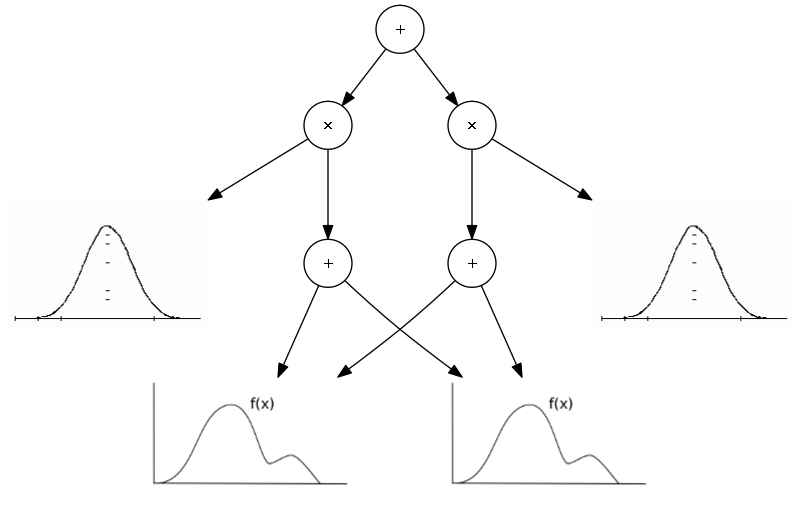
\includegraphics[scale=0.3]{graphs/alt_spn.png}
  \end{figure}
\end{frame}

\begin{frame}
  \frametitle{Uma visão mais intuitiva}
  \begin{description}
    \item[Nós internos:] variáveis latentes -- camadas ocultas:
    \begin{description}
      \item[$\oplus$:] mistura de distribuições -- ``semelhança entre instâncias'';
      \item[$\otimes$:] independência entre variáveis.
    \end{description}
    \item[Nós folhas:] Valoração/instanciação das variáveis.
  \end{description}\p
  \begin{figure}[h]
    \centering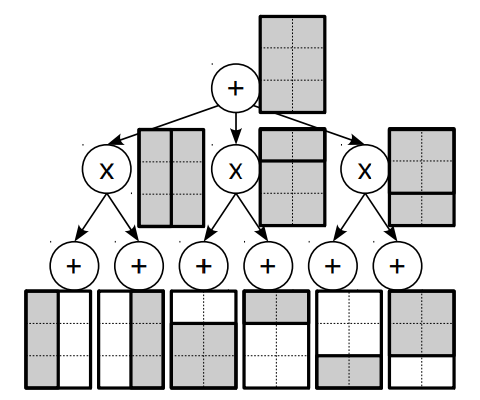
\includegraphics[scale=0.25]{imgs/img_spn.png}
    \caption{\textit{Learning the Structure of Sum-Product Networks Using Clustering on Variables},
      Dennis e Ventura~\cite{clustering}}
  \end{figure}
\end{frame}

\begin{frame}
  \frametitle{Inferência}

  \begin{figure}[h]
    \centering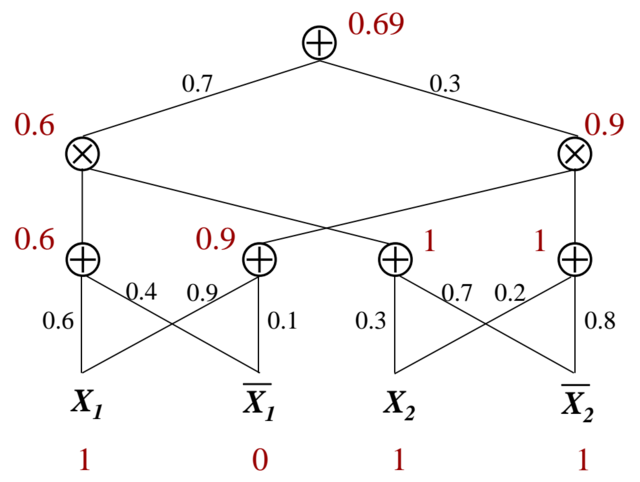
\includegraphics[scale=0.25]{imgs/marginals.png}
  \end{figure}
  \begin{equation*}
    \lambda_{X_1}=1,\lambda_{\overline{X}_1}=0,\lambda_{X_2}=1,\lambda_{\overline{X}_2}=1
  \end{equation*}
  \begin{equation*}
    S=\Pr(X_1=true)=f(x_1)=0.69
  \end{equation*}
\end{frame}

%--------------------------------------------------------------------------------------------------

\section{Aprendizado}

\begin{frame}
  \frametitle{Aprendizado}
  Queremos aprender uma SPN profunda.

  Lembrando$\ldots$

  \begin{description}
    \item[$+$] semelhanças nos dados
    \item[$\times$] independência entre variáveis
  \end{description}
\end{frame}

\begin{frame}
  \frametitle{Nós somas}
  Queremos achar \textit{clusters} de instâncias semelhantes: k-means clustering.

  \begin{figure}[h]
    \centering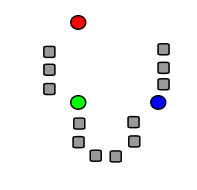
\includegraphics[scale=0.3]{imgs/kmeans0.png}
    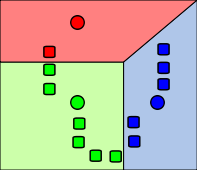
\includegraphics[scale=0.3]{imgs/kmeans1.png}
    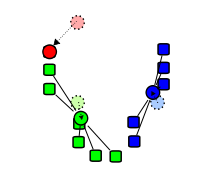
\includegraphics[scale=0.3]{imgs/kmeans2.png}
    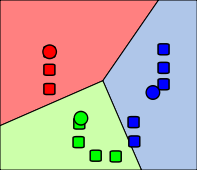
\includegraphics[scale=0.3]{imgs/kmeans3.png}
  \end{figure}

  Cada cluster $i=0..k-1$ será um filho de um nó soma.

  \textbf{Note:} todo filho tem mesmo escopo pois todo cluster tem mesmo escopo.
\end{frame}

\begin{frame}
  \frametitle{Nós produtos}
  Queremos achar conjuntos independentes de variáveis: grafo de independência.

  \begin{definition}
    Um grafo de independência é um grafo $G=(X,E)$ com variáveis $X$ como vértices e arestas
    $E=\{e_{ij} : X_i\text{---}X_j \iff X \not\perp Y\}$.
  \end{definition}

  Como testar independências par-a-par? Teste de independência por Chi-Quadrado ou por Entropia.

\end{frame}

\begin{frame}
  \frametitle{Nós produtos}
  \begin{proposition}
    Seja um grafo de independência $G=(X,E)$, os k-subgrafos $H_0,\ldots,H_k \subseteq G$
    desconexos tem escopos independentes par-a-par.
  \end{proposition}

  Cada subgrafo $H_i$ será um filho de um nó produto.

  \textbf{Note:} todo filho tem escopo disjunto de outro filho pois todo filho é independente
  par-a-par de seus irmãos.
\end{frame}

\begin{frame}
  \frametitle{Nós folhas}
  Queremos uma distribuição monovariável: contagem de frequências quando $|X|=1$.

  Considere um vetor $p$ onde cada índice $i=0,\ldots,n$ é uma possível valoração distinta e única
  de uma variável $X$ e que $X$ pode tomar até $n$ valorações diferentes. Dizemos que $p$ é então
  uma distribuição sobre $X$. Se $p$ obedece os axiomas da Teoria de Probabilidade, então $p$ é uma
  distribuição de probabilidade monovariável com domínio discreto.

  Seja um vetor $v$ de tamanho $k$ onde cada $v_i$ é uma valoração de $X$. Então $v$ é um vetor de
  frequência de $X$.

  Então $p$ será:
  \begin{equation*}
    p_i = \sum_{v_j = i} \frac{1}{k} = \Pr(X=i)
  \end{equation*}
\end{frame}

\begin{frame}
  \frametitle{Aprendizado estrutural de SPNs}
  \begin{algorithm}[H]
    \caption{LearnSPN~\cite{gens-domingos}}\label{learn-alg}
    \begin{algorithmic}[1]
      \Require~Conjunto $\set{X}$ de variáveis, conjunto $\set{I}$ de instâncias
      \Ensure~Uma SPN resultante do aprendizado estrutural
      \If{$|\set{X}|=1$}
        \State~Retorna uma distribuição monovariável de $\set{X}$
      \EndIf
      \State~Tente dividir as variáveis $\set{X}$ em $q$ partições $\set{X}_1,\ldots,\set{X}_q$
        onde $\set{X}_i$ é (aproximadamente) independente de todo $\set{X}_j$ para $i\neq j$.
      \If{dá para dividir}
        \State~\textbf{return} $\prod_{i=1}^q$ LearnSPN($\set{X}_i$, $\set{I}$)
      \Else
        \State~Divida as instâncias $\set{I}$ em partições $\set{I}_1,\ldots,\set{I}_k$ tal que
          $\set{I}_i$ seja uma coleção de instâncias mais similares possíveis entre si.
        \State~\textbf{return} $\sum_{i=1}^k \frac{|\set{I}_i|}{|\set{I}|}$ LearnSPN($\set{X}$,
          $\set{I}_i$)
      \EndIf
    \end{algorithmic}
  \end{algorithm}
\end{frame}

%--------------------------------------------------------------------------------------------------

\section{Código}

\begin{frame}
  \frametitle{Código}

  Se der tempo, agora vou mostrar o código. $\ddot\smile$
\end{frame}

%--------------------------------------------------------------------------------------------------

\section[Referências]{Referências e Bibliografia}
\begin{frame}[t,allowframebreaks]
  \frametitle{Referências e Bibliografia}
  \footnotesize
  \printbibliography[]
\end{frame}

\end{document}
